%%%%%%%%%%%%%%%%%%%%%%%%%%%%%%%%%%%%%%%%%
% Lachaise Assignment
% LaTeX Template
% Version 1.0 (26/6/2018)
%
% This template originates from:
% http://www.LaTeXTemplates.com
%
% Authors:
% Marion Lachaise & François Févotte
% Vel (vel@LaTeXTemplates.com)
%
% License:
% CC BY-NC-SA 3.0 (http://creativecommons.org/licenses/by-nc-sa/3.0/)
% 
%%%%%%%%%%%%%%%%%%%%%%%%%%%%%%%%%%%%%%%%%


%----------------------------------------------------------------------------------------
%	PACKAGES AND OTHER DOCUMENT CONFIGURATIONS
%----------------------------------------------------------------------------------------

\documentclass{article}

%%%%%%%%%%%%%%%%%%%%%%%%%%%%%%%%%%%%%%%%%
% Lachaise Assignment
% Structure Specification File
% Version 1.0 (26/6/2018)
%
% This template originates from:
% http://www.LaTeXTemplates.com
%
% Authors:
% Marion Lachaise & François Févotte
% Vel (vel@LaTeXTemplates.com)
%
% License:
% CC BY-NC-SA 3.0 (http://creativecommons.org/licenses/by-nc-sa/3.0/)
% 
%%%%%%%%%%%%%%%%%%%%%%%%%%%%%%%%%%%%%%%%%

%----------------------------------------------------------------------------------------
%	PACKAGES AND OTHER DOCUMENT CONFIGURATIONS
%----------------------------------------------------------------------------------------

\usepackage{amsmath,amsfonts,stmaryrd,amssymb} % Math packages

\usepackage{enumerate} % Custom item numbers for enumerations

\usepackage[ruled]{algorithm2e} % Algorithms

\usepackage[framemethod=tikz]{mdframed} % Allows defining custom boxed/framed environments

\usepackage{listings} % File listings, with syntax highlighting
\lstset{
	basicstyle=\ttfamily, % Typeset listings in monospace font
}

%----------------------------------------------------------------------------------------
%	DOCUMENT MARGINS
%----------------------------------------------------------------------------------------

\usepackage{geometry} % Required for adjusting page dimensions and margins

\geometry{
	paper=a4paper, % Paper size, change to letterpaper for US letter size
	top=2.5cm, % Top margin
	bottom=3cm, % Bottom margin
	left=2.5cm, % Left margin
	right=2.5cm, % Right margin
	headheight=14pt, % Header height
	footskip=1.5cm, % Space from the bottom margin to the baseline of the footer
	headsep=1.2cm, % Space from the top margin to the baseline of the header
	%showframe, % Uncomment to show how the type block is set on the page
}

%----------------------------------------------------------------------------------------
%	FONTS
%----------------------------------------------------------------------------------------

\usepackage[utf8]{inputenc} % Required for inputting international characters
\usepackage[T1]{fontenc} % Output font encoding for international characters

\usepackage{XCharter} % Use the XCharter fonts

%----------------------------------------------------------------------------------------
%	COMMAND LINE ENVIRONMENT
%----------------------------------------------------------------------------------------

% Usage:
% \begin{commandline}
%	\begin{verbatim}
%		$ ls
%		
%		Applications	Desktop	...
%	\end{verbatim}
% \end{commandline}

\mdfdefinestyle{commandline}{
	leftmargin=10pt,
	rightmargin=10pt,
	innerleftmargin=15pt,
	middlelinecolor=black!50!white,
	middlelinewidth=2pt,
	frametitlerule=false,
	backgroundcolor=black!5!white,
	frametitle={Command Line},
	frametitlefont={\normalfont\sffamily\color{white}\hspace{-1em}},
	frametitlebackgroundcolor=black!50!white,
	nobreak,
}

% Define a custom environment for command-line snapshots
\newenvironment{commandline}{
	\medskip
	\begin{mdframed}[style=commandline]
}{
	\end{mdframed}
	\medskip
}

%----------------------------------------------------------------------------------------
%	FILE CONTENTS ENVIRONMENT
%----------------------------------------------------------------------------------------

% Usage:
% \begin{file}[optional filename, defaults to "File"]
%	File contents, for example, with a listings environment
% \end{file}

\mdfdefinestyle{file}{
	innertopmargin=1.6\baselineskip,
	innerbottommargin=0.8\baselineskip,
	topline=false, bottomline=false,
	leftline=false, rightline=false,
	leftmargin=2cm,
	rightmargin=2cm,
	singleextra={%
		\draw[fill=black!10!white](P)++(0,-1.2em)rectangle(P-|O);
		\node[anchor=north west]
		at(P-|O){\ttfamily\mdfilename};
		%
		\def\l{3em}
		\draw(O-|P)++(-\l,0)--++(\l,\l)--(P)--(P-|O)--(O)--cycle;
		\draw(O-|P)++(-\l,0)--++(0,\l)--++(\l,0);
	},
	nobreak,
}

% Define a custom environment for file contents
\newenvironment{file}[1][File]{ % Set the default filename to "File"
	\medskip
	\newcommand{\mdfilename}{#1}
	\begin{mdframed}[style=file]
}{
	\end{mdframed}
	\medskip
}

%----------------------------------------------------------------------------------------
%	NUMBERED QUESTIONS ENVIRONMENT
%----------------------------------------------------------------------------------------

% Usage:
% \begin{question}[optional title]
%	Question contents
% \end{question}

\mdfdefinestyle{question}{
	innertopmargin=1.2\baselineskip,
	innerbottommargin=0.8\baselineskip,
	roundcorner=5pt,
	nobreak,
	singleextra={%
		\draw(P-|O)node[xshift=1em,anchor=west,fill=white,draw,rounded corners=5pt]{%
		Question \theQuestion\questionTitle};
	},
}

\newcounter{Question} % Stores the current question number that gets iterated with each new question

% Define a custom environment for numbered questions
\newenvironment{question}[1][\unskip]{
	\bigskip
	\stepcounter{Question}
	\newcommand{\questionTitle}{~#1}
	\begin{mdframed}[style=question]
}{
	\end{mdframed}
	\medskip
}

%----------------------------------------------------------------------------------------
%	WARNING TEXT ENVIRONMENT
%----------------------------------------------------------------------------------------

% Usage:
% \begin{warn}[optional title, defaults to "Warning:"]
%	Contents
% \end{warn}

\mdfdefinestyle{warning}{
	topline=false, bottomline=false,
	leftline=false, rightline=false,
	nobreak,
	singleextra={%
		\draw(P-|O)++(-0.5em,0)node(tmp1){};
		\draw(P-|O)++(0.5em,0)node(tmp2){};
		\fill[black,rotate around={45:(P-|O)}](tmp1)rectangle(tmp2);
		\node at(P-|O){\color{white}\scriptsize\bf !};
		\draw[very thick](P-|O)++(0,-1em)--(O);%--(O-|P);
	}
}

% Define a custom environment for warning text
\newenvironment{warn}[1][Warning:]{ % Set the default warning to "Warning:"
	\medskip
	\begin{mdframed}[style=warning]
		\noindent{\textbf{#1}}
}{
	\end{mdframed}
}

%----------------------------------------------------------------------------------------
%	INFORMATION ENVIRONMENT
%----------------------------------------------------------------------------------------

% Usage:
% \begin{info}[optional title, defaults to "Info:"]
% 	contents
% 	\end{info}

\mdfdefinestyle{info}{%
	topline=false, bottomline=false,
	leftline=false, rightline=false,
	nobreak,
	singleextra={%
		\fill[black](P-|O)circle[radius=0.4em];
		\node at(P-|O){\color{white}\scriptsize\bf i};
		\draw[very thick](P-|O)++(0,-0.8em)--(O);%--(O-|P);
	}
}

% Define a custom environment for information
\newenvironment{info}[1][Info:]{ % Set the default title to "Info:"
	\medskip
	\begin{mdframed}[style=info]
		\noindent{\textbf{#1}}
}{
	\end{mdframed}
}
 % Include the file specifying the document structure and custom commands

\usepackage{pgf}
\usepackage{booktabs}
\usepackage{graphicx}
\usepackage{listings}
\usepackage{hyperref}
\usepackage{wrapfig}
\usepackage{subcaption}
\usepackage{csquotes}
\usepackage{xcolor}

%----------------------------------------------------------------------------------------
%	ASSIGNMENT INFORMATION
%----------------------------------------------------------------------------------------

\title{Assignment 4: Fourth and Final Obligatory Exercise} % Title of the assignment

\author{Filip Stefaniuk\\ \texttt{filipste@student.matnat.uio.no}} % Author name and email address

%----------------------------------------------------------------------------------------

\begin{document}


\maketitle
\section{Introduction}
For this assignment, I have implemented Negation Resolution System, I started by creating simple baseline and
later extended it to make it similar to the one created by Fancellu \footnote{\href{http://www.aclweb.org/anthology/P16-1047}{Fancellu 2017}}.
Training and evaluation of the system can be easily done by running \lstinline{train.py} and \lstinline{eval.py}
scripts. Both of them support \lstinline{--help} command and are described in more detail in
\lstinline{README.md}. Data and error analysis were done in jupyter notebooks. Since evaluation
was done with external script I couldn't store the results in easily parsable file format, and metrics are
stored as txt files. All the code, data, metrics, notebooks, baseline and best negation cue detection model
are available in github repository\footnote{\href{https://github.uio.no/filipste/INF5820-Assignment4}{https://github.uio.no/filipste/INF5820-Assignment4}}.
\section{Preliminaries: Making Sense of the EPE File Format}


\subsection{Multiple negation instances}
Approach suggested in this exercise states that when more than one negation
cue appears in the sentence, it should be copied that many times witch each
negation cue and scope. To practice this approach, first exercise was to rewrite
a toy example in that manner. The result can be found in \lstinline{./data/toy_multiplied.tex}.

\subsection{Working with EPE structure}
To make working with the EPE structures simpler I have written Python class that embedds
sentences and allows to easily extract needed information. Note that no more additional
space or conversion is needed since the class stores all the data in the epe dictionary like
structure and the information is extracted dynamically. Class also have static method that
allows creating instances from json strings, thus loading epe file is simply calling this method
on each line of the file. Sentences may be converted to \lstinline{.tt} format by calling
\lstinline{to_tt()} method.

\subsection{Summary Statistics Extractions}
I have extracted requested statistics from all the available sentences (using both
training and developement set). Statistics below are computed for all the types of negation
cues and for multi-token and affix cues separately. Generally negation scope has on average
length of $8$. Number of negation tokens drops extremely quickly, to the point where most of
the negations occur only once.
When analysing the multi-token negation cues it is worth noticing,
that some of those have length equal 0, this is the case when the negation cue makes the whole sentence,
in example \textit{"By no means."}
\begin{figure}[h]
    \begin{subfigure}{0.5\textwidth}
        \centering
        \begin{tabular}{lllrr}
\toprule
{} &      tokens &   type &  mean scope len &  count \\
\midrule
0 &         not &    CUE &            8.55 &    398 \\
1 &          no &    CUE &            5.68 &    258 \\
2 &         n't &    CUE &            7.86 &     85 \\
3 &     nothing &    CUE &            7.15 &     71 \\
4 &       never &    CUE &            8.97 &     69 \\
5 &     without &    CUE &            4.39 &     31 \\
6 &        none &    CUE &            3.58 &     12 \\
7 &  impossible &  AFFIX &            8.09 &     11 \\
8 &         nor &    CUE &           14.80 &     10 \\
9 &      unable &  AFFIX &            7.25 &      8 \\
\bottomrule
\end{tabular}

    \end{subfigure}
    \begin{subfigure}{0.5\textwidth}
        \centering
        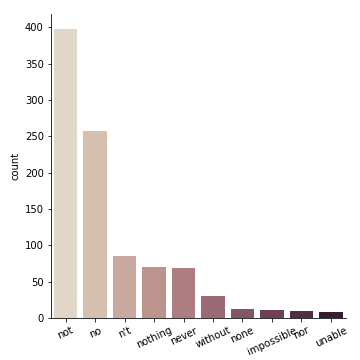
\includegraphics[scale=0.5]{../figures/negation_count.png}
    \end{subfigure}
    \caption{General statistics for negation cues.}
\end{figure}


\begin{figure}[h]
    \begin{subfigure}{0.45\textwidth}
        \centering
        \begin{tabular}{llrr}
\toprule
{} &             tokens &  mean scope len &  count \\
\midrule
0 &        neither/nor &             8.0 &      4 \\
1 &        by/no/means &             2.0 &      4 \\
2 &    on/the/contrary &             0.0 &      2 \\
3 &            not/not &            14.0 &      1 \\
4 &        rather/than &             8.0 &      1 \\
5 &     nothing/at/all &             0.0 &      1 \\
6 &  not/for/the/world &             0.0 &      1 \\
7 &             no/nor &             8.0 &      1 \\
8 &            no/more &             8.0 &      1 \\
\bottomrule
\end{tabular}

        \subcaption{multi-token negation cues}
    \end{subfigure}
    \hfill
    \begin{subfigure}{0.45\textwidth}
        \centering
        \begin{tabular}{llrr}
\toprule
{} &       tokens &  mean scope len &  count \\
\midrule
0 &   impossible &            8.09 &     11 \\
1 &       unable &            7.25 &      8 \\
2 &      unknown &            2.86 &      7 \\
3 &      unhappy &            4.83 &      6 \\
4 &     unlikely &           11.50 &      4 \\
5 &   unpleasant &            5.25 &      4 \\
6 &      useless &            7.25 &      4 \\
7 &   motionless &            3.00 &      3 \\
8 &  unambitious &            3.33 &      3 \\
9 &    imprudent &            5.33 &      3 \\
\bottomrule
\end{tabular}

        \subcaption{affix negation cues}
    \end{subfigure}
    \caption{count and mean scope length for 10 most frequent cues}
\end{figure}

\newpage
\section{A Joint Cue and Scope Sequence Tagger}
\subsection{End-to-end Negation Resolution System}
The Negation Resolution System that I have build uses Estimator class as a center point.
This class is responsible for building the model and provides interface to train and evaluate 
(it is convinient to use \lstinline{train.py} and \lstinline{eval.py} scripts). To transform
EPE sentenceces to data format that may be feed to keras classifier, estimator makes use of
preprocessor and postprocessor.
\paragraph{Preprocessor} extracts relevant information from the list of sentences,
builds numpy arrays of encoded input tokens, cue information and pos tags, with coresponding labels.
It does that in memory efficient manner by creating numpy arrays of fixed size and filling them with
relvant information.
\paragraph{Postprocessor} creates new list of sentences updated with list of given predicted labels.
To maintain compatibility with evaluation system, following heuristics are applied:
\begin{itemize}
\item when there is no negation cue in predicted tags for a given sentence, all the tokens are set to
out of negation scope token \textbf{T}
\item when all the tokens are predicted as \textbf{T} but there was a cue in input sentence,
\lstinline{negations} is set to 0 and \lstinline{negation} is removed from every node.
\item when token is predicted as affix tag \textbf{A}, lookup for this token is performed in the dictionary
of known affix cues. If the token is found, \textbf{negation} information is filled accordingly otherwise
the whole token is treated as a \textit{cue} and \textit{scope} is set to be an empty string.
\item \textit{event} value is copied from the input data.
\end{itemize}

\subsection{Evaluation of Baseline System}
I have evaluated baseline system using both LSTM and GRU recurrent neural network architectures.
I have used following setting:
\begin{itemize}
\item input was padded to length \textbf{100}
\item I have used randomly initialized word embeddings with size \textbf{300}.
\item Adam optimizer with learning rate \textbf{0.0001}
\item \textbf{200} neurons in recurrent neural network layer.
\item early stopping after \textbf{10} epochs without loss improvement on validation data.
\end{itemize}

\begin{wrapfigure}{r}{0.5\textwidth}
    \centering
    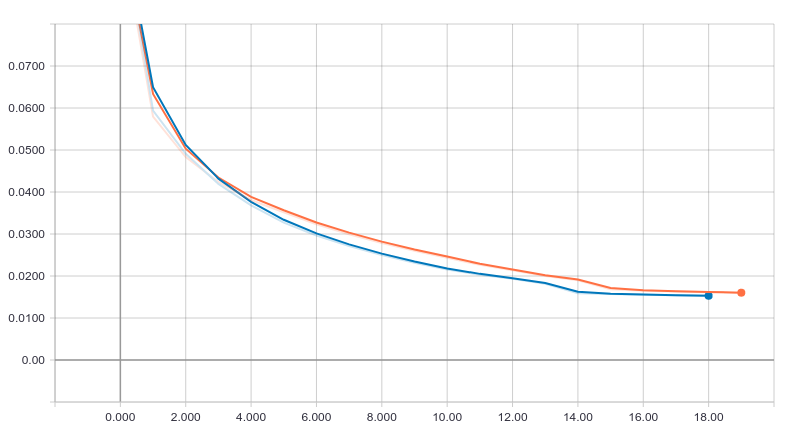
\includegraphics[scale=0.25]{../figures/loss.png}
    \caption {loss during training with LSTM (orange) and GRU (blue)}
\end{wrapfigure}

There wasn't much of a difference when training with GRU compared to LSTM.
On the plot to the right it is shown that the loss value was almost identical.
Training with LSTM was slightly slower (one epoch took ~50s compared to ~40s with GRU).
Scope token detection were better captured by GRU, but LSTM had better score on
cues detection.

\paragraph{Tag accuracy} because the classes were very unbalanced model had problems
with learning how to classify classes other that \textbf{T}. This is particulary visble
with Affix \textbf{A} class, where there were only 33 examples and not even one was classified
correctly.
\begin{figure}[h]
    \begin{subfigure}{0.45\textwidth}
        \centering
        \scalebox{0.8}{\begin{tabular}{lrrrr}
    \toprule
    {} &      precision &  recall &  f1-score & support \\
    \midrule
    True &         0.95 &    0.98 &      0.96 &   12758 \\
    False &        0.75 &    0.53 &      \textbf{0.62} &    1335 \\
    Cue &          0.73 &    0.85 &      \textbf{0.78} &     146 \\
    Affix Cue &    0.00 &    0.00 &      0.00 &      33 \\
    \bottomrule
    avg(micro) / total &  0.93 &    0.93 &      0.93 & 14272 \\
    avg(macro) / total &  0.61 &    0.59 &      0.59 & 14272 \\  
    \end{tabular}
    }
        \subcaption{LSTM}
    \end{subfigure}
    \hfill
    \begin{subfigure}{0.45\textwidth}
        \centering
        \scalebox{0.8}{\begin{tabular}{lrrrr}
    \toprule
    {} &      precision &  recall &  f1-score & support \\
    \midrule
    True &         0.95 &    0.98 &      0.97 &   12758 \\
    False &        0.80 &    0.55 &      \textbf{0.65} &    1335 \\
    Cue &          0.73 &    0.82 &      \textbf{0.77} &     146 \\
    Affix Cue &    0.00 &    0.00 &      0.00 &      33 \\
    \bottomrule
    avg(micro) / total &  0.93 &    0.94 &      0.93 & 14272 \\
    avg(macro) / total &  0.62 &    0.59 &      0.60 & 14272 \\  
    \end{tabular}
    }
        \subcaption{GRU}
    \end{subfigure}
    \caption{tagging accuracy}
    \end{figure}
\paragraph{*SEM 2012 Scorer} evaluation using official *SEM 2012 scorer yelded very similar results.
Score of \textit{Scope Tokens} that corresponds to \textit{False} if similar, I assume the 2\% difference
is caused by postprocessing heuristics. \textit{Cues} and \textit{Cue} tag have score difference of more
than 10\% this is caused by the fact that in tag evaluation affix cues are treated as a different class, and
in official scorrer they are counted as cues. Model predicts those cues very poorly, thus they lower the
overall score.

\begin{figure}[h]
\begin{subfigure}{\textwidth}
    \centering
    \begin{tabular}{lrrrrrrrr}
\toprule
{}           & gold & system &  tp &  fp &  fn & precision (\%) & recall (\%) & F1 (\%) \\
\midrule
Cues         &  173 &    142 &  94 &  18 &  79 &          83.93 &       54.34 &   \textbf{65.97} \\
Scope tokens & 1348 &    908 & 684 & 224 & 664 &          75.33 &       50.74 &   \textbf{60.64} \\
\bottomrule
\end{tabular}
    \subcaption{LSTM}
    \vspace*{3mm}
\end{subfigure}
\begin{subfigure}{\textwidth}
    \centering
    \begin{tabular}{lrrrrrrrr}
    \toprule
    {}           & gold & system &  tp &  fp &  fn & precision (\%) & recall (\%) & F1 (\%) \\
    \midrule
    Cues         &  173 &    132 &  87 &  15 &  86 &          85.29 &       50.29 &   \textbf{63.27} \\
    Scope tokens & 1348 &    907 & 715 & 192 & 633 &          78.83 &       53.04 &   \textbf{63.41} \\
    \bottomrule
\end{tabular}
    \subcaption{GRU}
\end{subfigure}
\caption{Evaluation results using official *SEM 2012 scorer}
\end{figure}

\section{Zooming in on Negation Scope}
\subsection{Differences between systems}
I have read the paper by Fancellu et al. and their code from github. It seems that their
experimental setup was slightly different than what we were supposed to do. First of all,
they used only sentences with at least one negation, which makes sence since it makes the token
classes a bit more balanced. Second they treated affix cue differently, instead of adding
a separate class they split them into \textit{cue} and \textit{scope} parts. Finally they focused
on predicting scope tokens and not cues, they added cue information to input data in form of an embedding.
\subsection{Evaluation of Negation System}
I tried to replicate the results achieved by Fancellu by making necessairy changes in my system.
I filtered the sentences and was left with \textbf{983} training samples and \textbf{173} validation samples.
Data split is a bit different to the one used by Fancellu (\textbf{848} training, \textbf{235} validation) but
I believe it is similar enough to produce comparable results. I have added cue information as an embedding
of size \textbf{50}. I used the same hidden size, learning rate, optimizer, max input length as in paper.
I have left affix cues as a separate class as instructed in the assignment.
I have trained and evaluated the system with different settings:
\begin{description}
\item[Cue info (C)] word embedding matrix randomly initialized and updated during training.
\item[External embeddings (E)] usage of external embeddings in non-static mode, I used 840B glove vectors.
\item[PoS information (PoS)] separate embedding for pos tags, initilized randomly and updated during trainig.
\end{description}

\begin{figure}[h]
\begin{tabular}{lrrrrrrrr}
    \toprule
    {}                   & gold & system &   tp &  fp &  fn & precision (\%) & recall (\%) & F1 (\%) \\
    \midrule
    BiLSTM - C           & 1348 &   1156 & 1054 & 102 & 294 &          91.18 &       78.19 &   84.19 \\
    BiLSTM - C + PoS     & 1348 &   1168 & 1069 &  96 & 279 &          91.76 &       79.30 &   \textbf{85.08} \\ 
    BiLSTM - C + E       & 1348 &   1215 & 1075 & 149 & 273 &          88.48 &       79.75 &   83.89 \\
    BiLSTM - C + E + PoS & 1348 &   1245 & 1084 & 161 & 264 &          87.07 &       80.42 &   83.61 \\
    \bottomrule
\end{tabular}
\caption{results of the scope detection}
\end{figure}

In comparison to Fancellu's system, mine performed worse (Fancellu achieved best F1 score \textbf{88.72}).
I believe the difference in the final results is caused by multiple minor differences, namely:
\begin{itemize}
\item the fact that in my system affix cues are treated differently
\item the datasets are not exactly the same
\item different word embeddings.
\item different postprocessing heuristics
\end{itemize}
\newpage
\section{Error Analysis: Looking on our Data}
\begin{wrapfigure}{r}{0.6\textwidth}
    \centering
    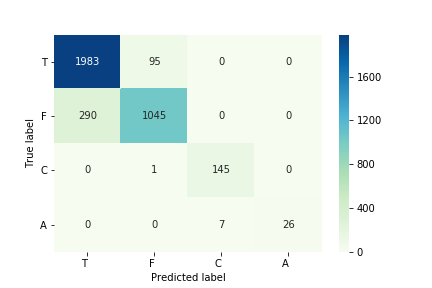
\includegraphics[scale=0.6]{../figures/confusion_matrix.png}
\end{wrapfigure}
I decided to perform error analysis on best model that is \textbf{BiLSTM - C + POS} similar to one done by Fancellu. I started
with plotting confusion matrix on tag level classification. Not suprisingly the model can distinguish
perfectly between negation cues and scopes, since we provide this information explicitly. It also looks
that it can distinguish quite well between affix and normal negation cues, and since the 3rd part of
this assignment was focused on detecting solely negation scopes I want to focus on that aspect in my further
analysis. Separately for \textbf{F} misclassified as \textbf{T} and \textbf{T} misclassified as \textbf{F}
I performed following analysis: I have selected sentences in which such misclassification occurs and sorted
them by the number of misclassified tokens. Then I highlighted all the scope tokens from the gold standard in \textcolor{blue}{blue}, then I highlighted correct predictions in \textcolor{teal}{green}
and misclassification in \textcolor{red}{red}. Finally I tried to find interesting classes of errors in those sentences.

\paragraph {Scope tokens missclassified as out of scope tokens} (59 sentences)\\
Often, espetially when it was more complex, subject was excluded from the negation scope (10 sentences):

\begin{displayquote}
The crime was ascribed to Nihilism, and \textcolor{blue}{the murderers were} \underline{never} \textcolor{blue}{arrested}.\\
The crime was ascribed to Nihilism, and \textcolor{red}{the murderers} \textcolor{teal}{were} \underline{never} \textcolor{teal}{arrested}.
\end{displayquote}
Another popular class of errors is when the negation scope continues after conjunction or punctuation (6 sentences):
\begin{displayquote}
I desire you to \textcolor{blue}{spare} \underline{no} \textcolor{blue}{expense and no pains to get at the truth}.\\
I desire you to \textcolor{teal}{spare} \underline{no} \textcolor{teal}{expense} \textcolor{red}{and no pains to get at the truth}.
\end{displayquote}
Systam also had problems with detecting discontinues scopes seperated by interjection (4 sentences):

\begin{displayquote}
\textcolor{blue}{It was} \underline{not}, I must confess, \textcolor{blue}{a very alluring prospect}. \\
\textcolor{teal}{it was} \underline{not}, I must confess, \textcolor{red}{a very alluring prospect}.

\end{displayquote}
    
\paragraph {Out of scope tokens classified as scope tokens} (34 sentences)\\
The negation scope was too wide
and included the word that connects to the next part of sentence (such as \textit{that} or \textit{since})
(3 sentences)
\begin{displayquote}
He says that \textcolor{blue}{they are} \underline{not} \textcolor{blue}{human}.\\
He says \textcolor{red}{that} \textcolor{teal}{they are} \underline{not} \textcolor{teal}{human}.
\end{displayquote}

Moreover system had problems with detecting scopes for affix cues with very little examples (most of them occured
only in one sentence or not at all in the trainig data) like: \textit{unburned}, \textit{inexplicable}, \textit{unbrushed}.
\newpage
\section{Further work}
I have a couple of ideas that one can implement to improve the performance of the system:
\paragraph{Affix cues:} Treating them as a different class, even though more linguistically correct
approach, seem not to improve results. I would argue that it even introduces undesirable noise since
the network needs to keep the information in its memory to distinguish between \textbf{A} and \textbf{C}
that seem not to contribute to scope detection. Since we still rely on the dictionary of known affix cues
in preprocessing, I would treat them as a normal cues during training.
\paragraph{Word Embeddings} In their work, Fancellu used custom word embeddings, it would be interesting
to train such model and experiment if it improves the results.
\paragraph{Dependency parsing information} Significant amount of errors are caused by model's inability to
distinguish the boundries of the noun and verb phrases. One could try to include encoded dependency tree information
to help model with this task, thus hopefully improving overall result.
\paragraph{Attention} It would be interesting to experiment with including attention mechanism, It could
help with capturing discontinues cues with the larger gaps between scopes.

\end{document}
